\documentclass[12pt,ngerman,titlepage,a4paper]{article}

\usepackage[utf8]{inputenc}
\usepackage{babel}
\usepackage{amsmath, amssymb, extarrows, amsthm} %einige hilfreiche Mathe-Pakete
\usepackage{graphicx, tikz} %Grafiken
\usepackage{yhmath}
\usepackage{mathtools}
\newtheorem{theorem}{Theorem}[section]
\newtheorem{lemma}[theorem]{Lemma}
\newtheorem{proposition}[theorem]{Proposition}
\newtheorem{definition}[theorem]{Definition}
\newtheorem{satz}[theorem]{Satz}
\newtheorem{fakt}[theorem]{Fakt}
\newtheorem{example}[theorem]{Beispiel}
\newtheorem{anmerkung}{Anmerkung}
\usepackage{hyperref}
\usepackage[figure]{hypcap}
\addto\captionsngerman{ 
	\renewcommand{\figurename}{Abb} 
}

\makeatletter
\newcommand*\bigcdot{\mathpalette\bigcdot@{.5}}
\newcommand*\bigcdot@[2]{\mathbin{\vcenter{\hbox{\scalebox{#2}{$\m@th#1\bullet$}}}}}

\makeatother

\DeclareMathOperator*{\argmin}{arg\,min}

\begin{document}

%===========================================================
\begin{titlepage}
\begin{center}

% TITEL
\textbf{\LARGE Contig-Assembly der MHC-Region mittels Linearer Programmierung}
%bei langen Titeln, die mehrere Zeilen benoetigen:
%\textbf{\LARGE Langer Titel der  ueber \medskip mehrere Zeilen laeuft}

\bigskip\bigskip
\textbf{Bachelorarbeit}
%bei Masterarbeit:
%\textbf{Masterarbeit}

\bigskip\bigskip\bigskip
Vorgelegt von

\bigskip
\textbf{Marvin Mischka Lindemann}

\bigskip
aus Berlin


\vfill
INSTITUT FÜR INFORMATIK\\
Algorithmische Bioinformatik\\
Universitätsstr. 1D–40225 Düsseldorf

\bigskip
%Abgabedatum:
tt.\ Monat jjjj

\bigskip
Betreuer: Prof.\ Dr.\ Gunnar W. Klau
%Wird der Schwerpunkt der Abschlussarbeit im Anwendungsfach gewaehlt:
%Betreuer: Prof.\ Dr.\ Vorname Nachname\\
%Zweitbetreuer: Prof.\ Dr.\ Vorname Nachname

\end{center}
\end{titlepage}

\thispagestyle{empty}\mbox{}\pagebreak
\setcounter{page}{0}

%===========================================================
\tableofcontents
\pagebreak

\section{Einleitung}
In dieser Bachelorarbeit möchte ich mithilfe von Linearer Programmierung APD-Contigs aus der MHC Region zu assemblieren.

WIKIPEDIA:
Der Haupthistokompatibilitätskomplex oder Hauptgewebeverträglichkeitskomplex (Abk. MHC von engl. major histocompatibility complex) umfasst eine Gruppe von Genen bei Wirbeltieren, die Proteine codieren, welche für die Immunerkennung, die Gewebeverträglichkeit (Histokompatibilität) bei Transplantationen und die immunologische Individualität wichtig sind. MHC-Regionen finden sich in allen Wirbeltieren ab den Knorpelfischen (Haie, Rochen). Beim Menschen sind diese Gene meist auf dem kurzen Arm von Chromosom 6 zu finden.[1]



\section{Grundlagen}
\subsection{Lineare Programmierung}

Die Problemstellung in dieser Arbeit lässt sich als lineares Programm formulieren. In der Linearen Programmierung möchten wir eine lineare Funktion maximieren oder minimieren, unter Berücksichtigung von linearen Ungleichungen welche die Funktionsparameter erfüllen müssen.
Formal mathematisch lässt sich dies so fassen:
\begin{align*}
	Gegeben:&\quad c \in \mathbb{R}^{n},\ A \in \mathbb{R}^{n \times m},\ b \in \mathbb{R}^{m} \\
	Gesucht:&\quad \argmin_{ x\in \mathbb{R}^n}\{c^Tx\,|\, Ax \leq b\}
\end{align*}
Dabei wird folgende Benennung verwendet:
\begin{description}
\item[\quad Variablen] $x_1,..., x_n$
\item[\quad Zielfunktion]  $c^Tx = \sum_{i=1}^n c_i x_i$
\item[\quad Bedingungen]  $Ax \leq b = \sum_{i=1}^n a_{ji} x_i \leq b_j, \ j = 1,...n$
%Dabei wird $c^Tx = \sum_{i=1}^n c_i x_i$ die Zielfunktion genannt und $Ax \leq b = \sum_{i=1}^n a_{ji} x_i \leq b_j, \ j = 1,...n$ Bedingungen.
\end{description} Das folgende Beispiel illustriert diese Definition:
\begin{example}
	gutes Beispiel Ausdenken
\end{example}

\subsection{Contig-Assembly}
Bei einem \emph{Contig-Assembly} wird versucht eine DNA Sequenz zusammenzubauen aus vielen kleineren Stücken genannt \emph{Contigs}. Contigs sind dabei Zusammenhängende DNA-Stränge die mit hoher Wahrscheinlichkeit in der fertigen Sequenz so vorkommen. Für den Zusammenbau verwendet man Informationen aus \emph{Constraints}, ein Constraint gibt eine vermutete Distanz zwischen zwei Contigs an.\\
Ein \emph{Repeat} ist ein Contig, der an mehreren Stellen in der DNA Sequenz vorkommt.

\section{Ausgangslage}

Es liegen zwei Dateien vor, einmal eine Liste von allen Contigs von APD und deren Länge. Sowie eine Datei mit Constraints. Diese Constraints sind wie folgt aufgebaut:
\begin{align*}
&a \quad b \quad 1000\\
&a \quad b \quad 1100\\
&b \quad c \quad 3000\\
&a \quad c \quad 6000
\end{align*}
Dabei sind die ersten beiden Spalten zwei Contigs und die dritte die Entfernung vom rechten Rand des ersten Contigs zum linken Rand des zweiten Contigs. Die Constraints können nun einige Widersprüche aufweisen. Diese können in drei Kategorien eingeteilt werden. 
\begin{enumerate}
\item Ungenauigkeiten beim Messen oder kleinere Indels
\item falsche Constraints
\item Repeats
\end{enumerate}
Im folgenden wollen wir die Repeats identifizieren um so eine Lösung zu finden die möglichst viele Constraints erklärt.
\section{Vorgehen}
Wir werden nun die Contigs mit linearer Programmierung positionieren und dann versuchen ein Repeat zu identifizieren und aufzuteilen. Dies wiederholen wir Schrittweise bis kein Repeat mehr ausgemacht werden kann.
\subsection{Vorbereitung}
Vor dem eigentlichen Lösen, habe ich die Constraints mithilfe der Längen-Datei so umgeändert, dass die Entfernung immer bezüglich dem linken Rand des ersten Contigs zum linken Rand des zweiten Contigs ist, indem ich die Länge des ersten Contigs zu der Entfernung addiert habe.\\
Nun habe ich überprüft, ob die Constraints ein zusammenhängendes Gen darstellen. Dazu habe ich in einer Union-find-Datenstruktur jedes Contig in einer Menge gespeichert und die Mengen der Contigs vereinigt, wenn es ein Constraint mit diesen beiden gab.
Bei unzusammenhängenden Daten habe ich mit der größten Zusammenhangskomponente weitergemacht.

\subsection{Notationen}
Im Folgenden bezeichnet $D$ die Multimenge aller Constraints und $C$ die Menge aller Contigs.
\subsection{Assembly}
\subsubsection*{LP Lösen} Wir möchten die Contigs so positionieren, dass der durchschnittliche Fehler aller Constraints möglich klein ist:
%\[ pos = \argmin_{pos': C \rightarrow \mathbb{N}} \left\{ \sum_{(a,b,dist) \in D} |pos'(b) - pos'(a) - dist| \right\}\]
%$\mathbb{pos}$\\$\mathbf{pos}$\\$\mathcal{pos}$\\$\mathfrak{pos}$\\$\mathit{pos}$\\$\mathrm{pos}$\\$\mathsf{pos}$\\$\mathtt{pos}$\\
\[ pos = \argmin_{pos': C \rightarrow \mathbb{N}} \ \sum_{(a,b,dist) \in D} |pos'(b) - pos'(a) - dist| \]
Um daraus ein lineares Programm zu machen, führen wir für jeden Constraint $(a,b,dist)$ aus $D$ eine Hilfsvariable $\varepsilon$ ein mit:
\begin{align*}
 \varepsilon &= |pos(b) - pos(a) - dist|\\
  &= \max \{pos(b) - pos(a) - dist, -pos(b) + pos(a) + dist \} 
\end{align*}
somit ist $\varepsilon$ die kleinste Zahl die größer oder gleich $pos(b) - pos(a) - dist$ und $-pos(b) + pos(a) + dist$ ist. Daraus folgt dass folgendes lineares Programm die optimale Positionierung berechnet:
\begin{align*}
	\text{Variablen:}\quad& pos(c) \ \forall c \in C \ \ \text{und} \ \ \varepsilon_{d}  \ \forall \ d \in D\\
	\text{Zielfunktion:}\quad& \sum_{d \in D} \varepsilon_{d}\\
	\text{Bedingungen:}\quad \begin{split} pos(b) - pos(a) - dist \leq \varepsilon_{d}\\
	                                      -pos(b) + pos(a) + dist \leq \varepsilon_{d} \end{split}\quad \forall \ (a,b,dist) = d \in D
\end{align*}
Die Positionen sind eigentlich Natürliche Zahlen, da sie die Anzahl der Basenpaare angeben, wie weit die Constraints voneinander entfernt sind. Das Lösen eines Linearen Programms mit natürlichen Variablen benötigt ungleich länger als mit reellen Variablen und die Distanzwerte weisen sowieso zu große Schwankungen auf um auf den Basenpaar genau zu sein. Daher bietet es sich an, die Relaxierung des LP zu betrachten, also auch reelle Positionen zuzulassen.
Wir lösen dieses Lineare Programm mithilfe von Gurobi.
\subsubsection*{Repeat finden} 
Als nächsten Schritt erstellen wir eine Liste für jeden Contig, in der pro Constraint in dem der Contig enthalten ist ein Wert gespeichert wird, wir stark der Constraint verletzt wird. So wird für Contig $b$ mit diesen Constraints und dieser Positionierung
\begin{align*}
&a \quad b \quad 1000 &&pos(a) = 10000\\
&a \quad b \quad 1100 &&pos(b) = 11000\\
&b \quad c \quad 3000 &&pos(c) = 14000\\
&b \quad c \quad 6000
\end{align*}
diese Liste $[0, 100, 0, -3000]$ erstellt. Es steht also für jeden Constraint ein Wert in der Liste, der angibt um wie viele Basenpaare man $b$ verschieben müsste, damit dieser Constraint erfüllt wäre, wenn der Contig im Constraint die Position behält.
Nun clustern wir die Werte in der Liste, und berechnen einen Güte-Wert wie gut man aus den Fehlern auf einen Repeat schließen kann.
Angenommen wir haben diese sortierte Fehler-Liste für ein Contig:
{\footnotesize \[ {-8000} \ \ {-340} \ \ {-200} \ \ {-100} \ \ {-60} \ \ {-30} \ \ {-30} \ \ {-10} \ \ 0 \ \ 40 \ \ 100 \ \ 5450 \ \ 6000 \ \ 6200 \ \ 6300 \ \ 6500\]}
Dann würde zuerst alles was weniger als 500 Basenpaare Unterschied hat, in eine Gruppe unterteilt:
{\footnotesize \[ {-8000} \, | \, {-340} \ \ {-200} \ \ {-100} \ \ {-60} \ \ {-30} \ \ {-30} \ \ {-10} \ \ 0 \ \ 40 \ \ 100 \, | \, 5450 \,| \, 6000 \ \ 6200 \ \ 6300 \ \ 6500\]}
Sei $G_1$ die Gruppe mit den meisten Einträgen und $G_2$ die Gruppe mit dem zweitkleinsten Einträgen und $R$ alle Werte die weder in $G_1$ noch in $G_2$ sind, dann wird die Güte wie folgt bestimmt:
\[\frac{|G_2|^2 \, log_2( |mean(G_2) - mean(G_1)| - 499 )}{1 + |G_2| + |R| }\]
In unserem Beispiel also:
\[\frac{4^2 \, log_2( |6250 - (-63)| - 499 )}{1 + 4 + 2 } \approx 28.58\]
Danach wird geschaut, ob man durch einen größeren Gruppierungswert als 500 eine bessere Güte erreichen kann, indem schrittweise nahe Gruppen vereinigt werden. In unseren Beispiel sind die beiden Gruppen mit dem kleinsten Abstand die 5450 mit der Nachfolgenden Gruppe.
{\footnotesize \[ {-8000} \, | \, {-340} \ \ {-200} \ \ {-100} \ \ {-60} \ \ {-30} \ \ {-30} \ \ {-10} \ \ 0 \ \ 40 \ \ 100 \, | \, 5450 \ \ 6000 \ \ 6200 \ \ 6300 \ \ 6500\]}
\[\frac{5^2 \, log_2( |6090 - (-63)| - 549 )}{1 + 5 + 1 } \approx 44.47\]
Als letztes würden die beiden großen Gruppen vereinigt.
{\footnotesize \[ {-8000} \, | \, {-340} \ \ {-200} \ \ {-100} \ \ {-60} \ \ {-30} \ \ {-30} \ \ {-10} \ \ 0 \ \ 40 \ \ 100 \ \ 5450 \ \ 6000 \ \ 6200 \ \ 6300 \ \ 6500\]}
\[\frac{1^2 \, log_2( |-8000 - 1988| - 5349 )}{1 + 1 + 0 } \approx 6.09\]
Damit ergibt sich, dass das mit Güte 44.47 davon ausgegangen werden kann, dass das es 2 Repeat-Versionen von diesem Contig gibt, eine um 63 Basenpaare nach links verschoben und eine 6090 Basenpaare weiter rechts. Ist dies die größte Güte von allen Contigs, dann wird der Contig durch diese beiden Versionen ausgetauscht. Schließlich wird der Contig in allen Constraints durch die Repeat-Version ausgetauscht, welche den kleinsten den kleineren Fehler für diesen Constraint aufweist.
Wird also Contig $b$ aufgeteilt in $b_1$ und $b_2$ mit
\begin{align*}
&a \quad b \quad 1000 &&pos(a) = 10000\\
&a \quad b \quad 1100 &&pos(b_1) = 11000\\
&b \quad c \quad 3000 &&pos(b_2) = 8000\\
&b \quad c \quad 6000 &&pos(c) = 14000
\end{align*}
so resultieren dann die Constraints
\begin{align*}
&a \quad b_1 \quad 1000 &&\phantom{pos(a) = 10000}\\
&a \quad b_1 \quad 1100\\
&b_1 \quad c \quad 3000\\
&b_2 \quad c \quad 6000
\end{align*}

\subsubsection*{Widerholung} 
Dieses Prozedere wird nun wiederholt, dabei kommen aber ein kleiner zusätzlicher Aspekt hinzu.
Nach dem das LP erneut gelöst wurde, wird vor dem bestimmen der Fehler-Listen der Contigs erst für jeden Constraint überprüft,
ob nicht eine andere Contig-Version zugeordnet werden sollte.
Dafür werden alle Repeat-Versionen der beiden beteiligten Contigs paarweise überprüft.
so könnte $(a_1,b_3,1100) \in D$ als Constraint vorkommen und dann durch $(a_2,b_2,1100)$ ausgetauscht werden, wenn dies den kleinsten Fehler in der Positionierung ergibt. Dadurch behindert eine frühere falsche Zuordnung von Repeat-Versionen nicht den weiteren Algorithmus.
Bei jedem Durchlauf wird die Positionierung abgespeichert, so dass an einem beliebigen Zeitpunkt abgebrochen werden kann und das letzte Ergebnis noch vorhanden ist. Ansonsten terminiert der Algorithmus sobald ein festgelegter Gütewert unterschritten wird.

\section{Auswertung}
99.86\% der Contigs sind Teil der größten Zusammenhangskomponente. Das heißt 3 von 2124 Contigs sind nicht Teil eines Constraints mit irgendeinem anderen der 2121 Contigs.\\
Pro Durchlauf (also pro gefundenen Repeat) benötigt der Algorithmus zwischen 30 und 60 Sekunden (Daten des PC hier einfügen?) Davon wird über die Hälfte für das Lösen des Linearen Programms benötigt.\\
Es gibt keinen großen sprunghaften Abfall der Gütefunktion an irgendeiner bestimmten Stelle, wodurch es schwer ist eine Grenze zu ziehen, wann die Datenlage noch für ein Repeat spricht und ab wann es andere Erklärungen für die Datenlage gibt.
In der Abbildung \ref{fig:gute} wird gezeigt wie sich die Güte im laufe der ersten 50 Repeats entwickelt.
\begin{figure} 
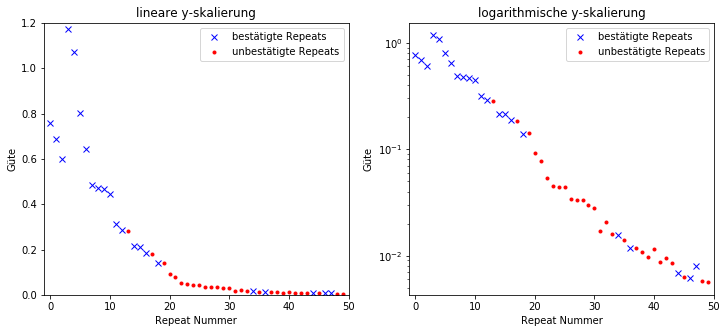
\includegraphics[width=1\textwidth]{gute}
\caption{Verlauf der Gütefunktion}%
\label{fig:gute}
\end{figure}
Als Referenz wie schlüssig die Repeats sind, wurde ein Assembly als Vergleich verwendet, welches vom Institut für Medizinische Mikrobiologie und Krankenhaushygiene der HHU stammt.
Dabei wurden 44 Repeats gefunden von denen 22 auch in unserer Auswertung der ersten 50 Repeats enthalten sind. Die ersten 12 gefundenen Repeats sind alle bestätigt, danach kommt es immer öfter zu anderen Ergebnissen. Wie kann es zu dieser Abweichung kommen? Ein Hinweis darauf gibt die Länge des assemblierten Stangs. Dieser beträgt knapp über 3 Millionen Basenpaare, anstatt ungefähr 4.9 Millionen Basenpaare. Der Strang ist also deutlich zu kurz. Die Ursache daran erkennt man in folgender grafischen Darstellung \ref{fig:d3} des Assmebly als Graph.

\begin{figure} 
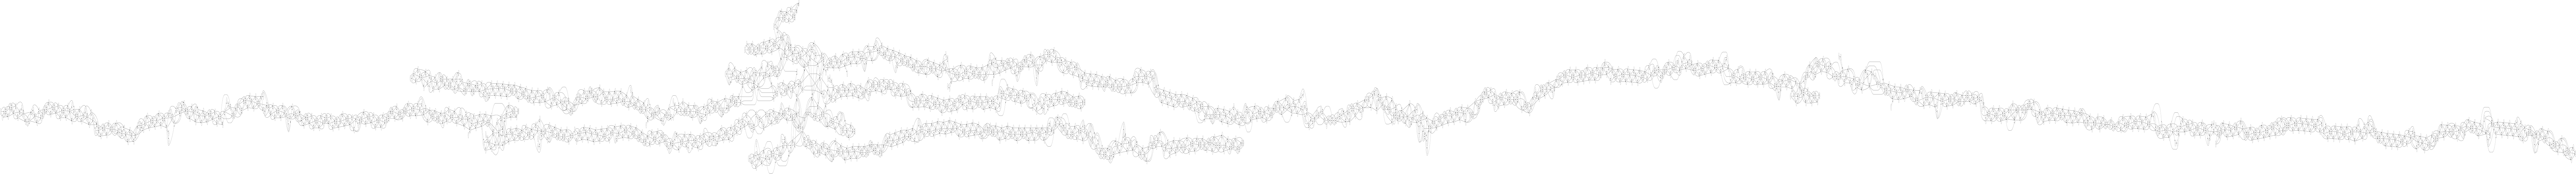
\includegraphics[width=1\textwidth]{test}
\caption{kompletter Assambly}%
\label{fig:dd}
\end{figure}
\begin{figure} 
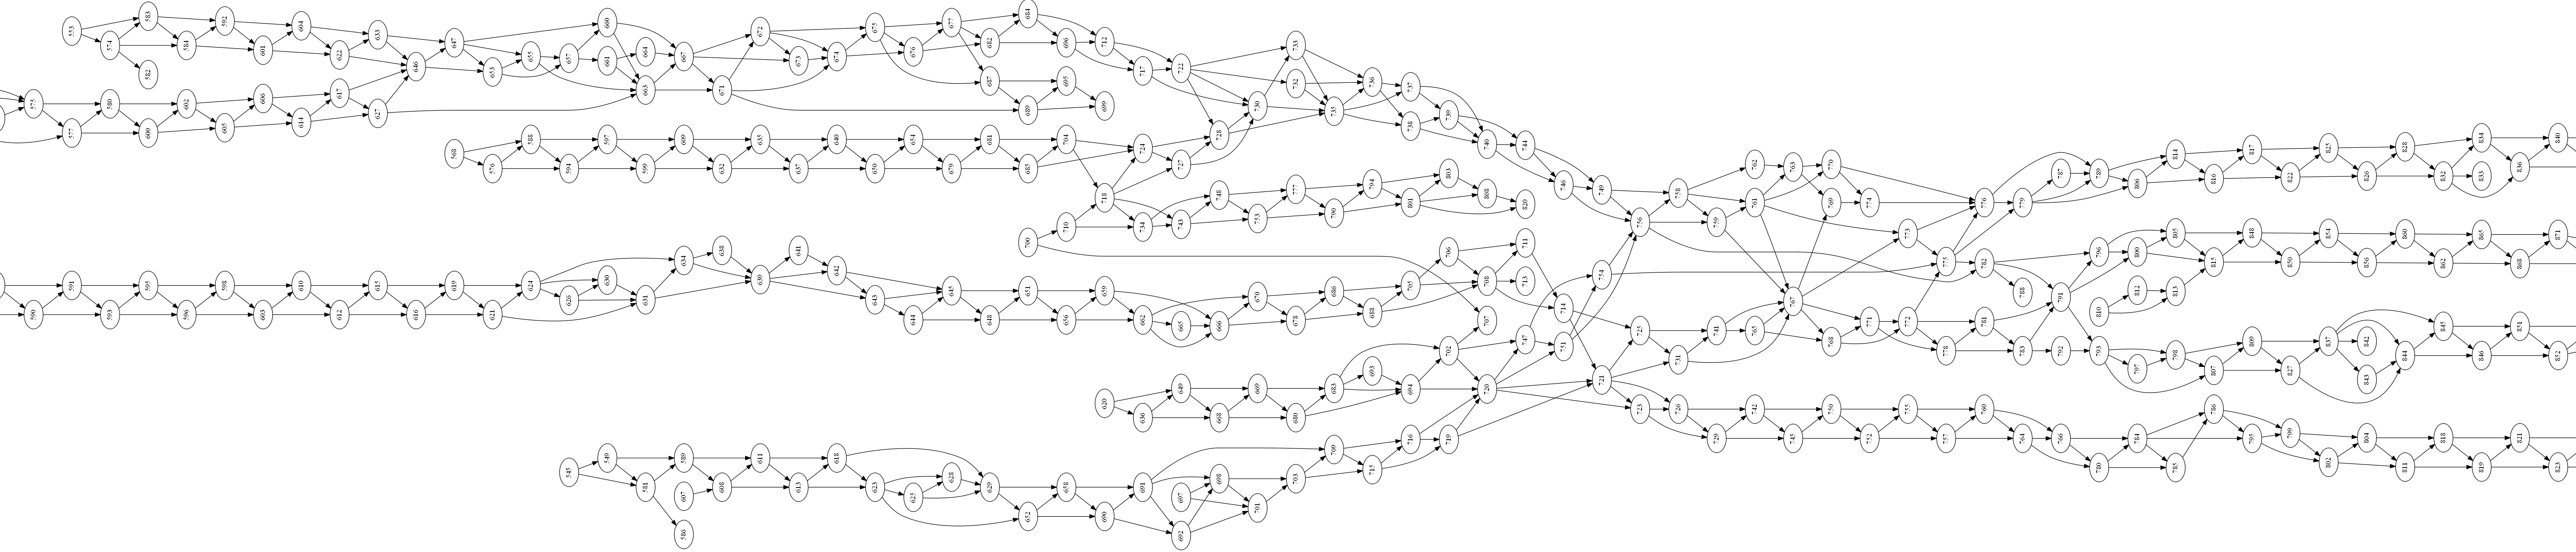
\includegraphics[width=1\textwidth]{d33}
\caption{vergrößerter Ausschnitt}%
\label{fig:d3}
\end{figure}

Für jeden Contig gibt es einen Knoten. Die Nachbarschaft eines Contigs $a$ wird bestimmt, indem alle Contigs betrachtet werden, welche mit $a$ in einem Constraint enthalten sind, dessen Fehler kleiner als 1000 Basenpaare bezüglich der Positionierung ist. Von diesen Contigs werden die beiden mit der höchsten Positionierung vor $a$ als Vorgänger und die beiden mit der kleinsten Positionierung hinter $a$ als Nachfolger von $a$ gesetzt. Idealerweise würde man eine Zick-Zack-Leiter als Muster erwarten wie sie auch auf kurzen Stücken zu erkennen ist. Kleine Abweichungen vom Muster liegen an zwei Contigs die obwohl sie nah aneinander liegen kein Constraint haben. Das aber komplette Stränge getrennt nebeneinander laufen ist unrealistisch.\\
Wir müssten als das Lineare Programm dazu bringen, dass es nur sehr ungern Contigs nah aneinander positioniert, zwischen denen es kein Constraint gibt. Dies ist aber nicht ohne weiteres möglich, da wir mit dem Linearen Programm nur ausdrücken können, dass ein Contig weit vor einem anderen Contig sein muss, aber nicht, dass es entweder weit vor, oder weit hinter einem anderen Contig sein muss, also weit entfernt.


%===========================================================
\pagebreak\noindent

\textbf{\LARGE Erkl\"arung}
\addcontentsline{toc}{section}{Erkl\"arung}

\bigskip\bigskip
\noindent 
Hiermit versichere ich, dass ich die   Bachelorarbeit selbst\"andig verfasst und keine
anderen als die angegebenen Quellen und Hilfsmittel benutzt habe.

\bigskip
\noindent
D\"usseldorf, den tt.\ Monat jjjj

\bigskip\bigskip\bigskip
\noindent
(Vorname Nachname)

\end{document}

